\chapter{Background} \label{chap:background} \minitoc

\section*{}


This chapter describes the necessary foundations regarding visual programming tools for the Internet-of-Things context. Section~\ref{sec:background_iot} describes the background of the Internet-of-Things paradigm and important concepts in that area, with a description of IoT architectures, including Fog and Edge, in Section~\ref{sec:architectures}. Section~\ref{sec:node-red} describes the Node-RED programming tool and its architecture and uses. Finally, Section~\ref{sec:background_vpl} mentions visual programming languages, their uses as well as their benefits and drawbacks.

\section{Internet-of-Things}\label{sec:background_iot}

Internet-of-Things paradigm was defined by the committee of the International Organization for Standardization and the International Electrotechnical Commission~\cite{ISOIEC} as:
\begin{quote}
    \emph{“An infrastructure of interconnected objects, people, systems and information resources together with intelligent services to allow them to process information of the physical and the virtual world and react.”}
\end{quote}

This paradigm is built upon the network of heterogeneous devices interconnected between themselves, people and the environment. According to Buuya~\cite{iot_future_direction}, the applications of IoT systems can be divided into four categories: (i)~Home at the scale of an individual or home, (ii)~Enterprise at the scale of a community, (iii)~Utilities at a national or regional scale and (iv)~Mobile, which is spread across domains due to its large scale in connectivity and scale. 
%Nowadays, the use of Internet-of-Things systems is present in different areas, such as aerospace, automotive, telecommunications and health industries, as well as city and agriculture managements, amongst others \cite{applications_iot}.

However, one might think that IoT only relates to machines and interactions between them. Most of the devices we use in our day-to-day - mobile phones, security cameras, watches, coffee machines - are now computation capable of making moderately complex tasks and are constantly generating and sending information. This relates to the \emph{human-in-the-loop} concept, where humans and machines have a symbiotic relationship~\cite{human_in_the_loop_survey}.
 
\subsection{IoT architectures}\label{sec:architectures}

Internet-of-Things systems deal with big amounts of data from different sources and have to process it in efficient and fast ways. Typical IoT systems are composed of three tiers, which are:

\begin{itemize}
    \item \textbf{Cloud Tier}, which is composed of data centers and servers, normally running remotely. It is characterized by having high computation power and latency.
    \item \textbf{Fog Tier} is composed of gateways and devices that are normally between the cloud servers and the edge devices. This tier has less latency than the cloud, more heterogeneity, and geographical distribution.
    \item \textbf{Edge Tier} contains all the edge devices (sensors, embedded systems, light sources, etc). Since its devices have smaller computational capabilities, this tier is the one with smaller computation power but with less latency value.
\end{itemize}

These tiers can also be called Application Layer, Network Layer, and Perception Layer~\cite{iot_layers}, respectively, which is compatible with the characterizing mentioned above. However, not all devices in each tier map to the respective layer. One example is a third-party service that gives readings. It can be contained in the Perceptive Layer, but it is not included in the Edge Tier.

New paradigms of computing appeared related to each of these tiers. The majority of IoT systems use a Cloud Computing architecture, where it takes advantage of centralized computing and storage. This approach has several benefits, such as increased computational capabilities and storage, as well as easier maintenance. However, it comes with several problems such as (a) high latency and (b) high use of bandwidth, due to the need to send the data generated from the sensors to the centralized unit~\cite{connecting_fog_and_cloud}. Systems that only use cloud computing are not scalable, specially real-time applications, which are sensitive to increased latency. With the increasing computation capabilities of edge devices and the requirements of reduced latency, two new paradigms appeared - Fog and Edge Computing.

\subsubsection{Fog Computing}\label{sec:fog_computing}

Nowadays, with the improvement of wireless networks and the hardware and software of mobile devices, there is a possibility to take advantage of these variables in the computational execution of IoT systems. This will allow for devices in the network to communicate and share resources between them, reducing latency. The central instance, which in the paradigm before executed all the computation, now serves as a scheduler and state manager of the communication between the devices, occasionally providing necessary resources if needed. The paradigm described before is called Fog Computing, which aims to bring computing closer to the perception tier, bringing the cloud near the edge of the network~\cite{mobile_cloud}. It focuses on distributing data throughout the IoT system, from the cloud to the edge devices, making the system a distributed one.

According to Buuya~\cite{IoT_principles_and_paradigms}, Fog Computing has several advantages: (i)~reduction of network traffic by having edge devices filtering and analyzing the data generated and sending data if necessary, (ii)~reduced communication distance by having the devices communicate between them without using the cloud as middleman, (iii)~low-latency by moving the processing closer to the data source rather than communicating all the data to the cloud for it to be processed, and (iv)~scalability by reducing the burden on the cloud, which could be a bottleneck for the system.

It is possible to see an example of the architecture of an IoT system using the Fog paradigm in Figure \ref{fig:fog_architecture}. The Fog Computing connects the cloud to the edge devices, normally with the use of access points and gateways. 

\begin{figure}[h]
\centering
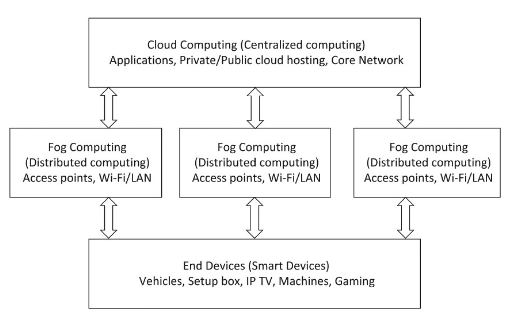
\includegraphics[width=0.8\textwidth]{fog_computing_architecture.png}
\caption[Fog Computing Architecture]{Fog Computing Architecture~\cite{IoT_principles_and_paradigms}}
\label{fig:fog_architecture}
\end{figure}

Despite all the advantages, Fog Computing has several requirements and difficulties. To make a successful and efficient distribution of computation and communication, it requires knowledge about the resources of the connected devices. The complexity is also bigger than Cloud Computing since it needs to work with heterogeneous devices with different capacities. 
       
\subsubsection{Edge Computing}\label{sec:edge_computing}

Edge Computing, also known as Mist Computing, is a distributed architecture that uses the devices' computational power to process the data they collect or generate. It takes advantage of the Edge tier, which contains the devices closer to the end-user - smartphones, TVs, sensors, etc. The goal of this paradigm is to minimize the bandwidth and time response of IoT systems while leveraging the computational power of the devices in them. It reduces bandwidth usage by processing data instead of sending it to the cloud to be processed, which is also correlated to reduced latency since it does not wait for the server response. In addition to these advantages and related to their cause, Edge Computing also prevents sensitive data from leaving the network, reducing data leakage and increasing security and privacy~\cite{edge_computing, edge_computing_2019}.

In this paradigm, each device serves both as a data producer and a data consumer. Since each device is constrained in terms of resources, this brings several challenges such as system reliability and energy constraints due to short battery life and overall security. Other issues consist of the lack of easy-to-use tools and frameworks to build cloud-edge systems, non-existent standards regarding the naming of edge devices and the lack of security edge devices have against outside threats such as hackers~\cite{promise_of_edge_computing}.

There is some confusion in the research community regarding the concepts of Fog and Edge computing. The publication from Iorga et. al.~\cite{fog_edge_differences} was used to inspire the definitions of these terms in this dissertation. Edge Computing focuses on executing applications in constrained devices, without worrying about storage or state preservation. On the other hand, Fog Computing is hierarchical and includes devices with more capabilities, capable of control activities, storage, and orchestration.

\section{Visual Programming Languages}\label{sec:background_vpl}

Visual Programming, as defined by Shu, consists of using meaningful graphical representations in the process of programming~\cite{vpl_definition_shu}. With this definition, we can consider Visual Programming Languages (VPLs) as a way of handling visual information and interaction with it, allowing the use of visual expressions for programming. According to Burnet and Baker~\cite{scaling_vpls}, visual programming languages are constructed to \emph{"improve the programmer's ability to express program logic and to understand how the program works"}.

There are several applications of visual programming languages in different areas, such as education, video game development, automation, multimedia, data warehousing, system management, and simulation, with this last area being the area with most use cases~\cite{survey_vpl_iot}.

Visual programming languages have several characteristics, such as a concrete process and depiction of the program, immediate visual feedback and requires the knowledge of fewer programming concepts (e.g. pointers, memory allocation, etc)~\cite{scaling_vpls}.

VPLs were categorized by Downes~\cite{vpls_survey} based on their visual paradigms and architecture: 
\begin{itemize}
    \item \textbf{Purely Visual Languages}, where the creation is made using only graphical elements and the subsequently debugging and execution is made in the same environment.
    \item \textbf{Hybrid text and visual systems}, where the programs are created using graphical elements but their executions is translated into text language.
    \item \textbf{Programming-by-example systems}, where a user uses graphical elements to teach the system.
    \item \textbf{Constraint-oriented systems}, where the user translates physical entities into virtual objects and applies constraints to them, in order to simulate their behavior in reality.
    \item \textbf{Form-based systems}, which were based on the architecture and behavior of spreadsheets.
\end{itemize}
The categories mentioned can be present in a single system, making them not mutually exclusive.

\section{Node-RED}\label{sec:node-red}

Node-RED~\cite{node_red} is a programming tool applied to the development of Internet-of-Things systems. It was first developed with to manipulate and visualize mappings between MQTT topics in IBM's Emerging Technology Services group. It then expanded into a more general open-source tool, which is now part of the JS Foundation.

It is a web-based tool consisting of a run time built with the Node.js framework and a browser-based visual editor. This tool provides the end-user with a simple interface to connected devices and APIs, using a flow-programming approach. Programs are called \emph{flows}, built with \emph{nodes} connected by wires. Each node corresponds to an action, such as input, output, data processing, etc.

The Node-RED interface has three components: (1)~Palette, (2)~Workspace and (3)~Sidebar. The Palette contains all the nodes installed and available to use, divided into categories. They can be used by dragging them into the workspace and additional features for each node are accessible by double-clicking them. The Workspace is where the flows are created and modified. It is possible to have several \emph{flows} and \emph{sub-flows} accessible with the use of tabs. Lastly, the Sidebar contains information about the nodes, the debug console, node configuration manager and the context data. Figure \ref{fig:node_red_window} showcases the visual interface of Node-RED and its elements.

\begin{figure}[h]
\centering
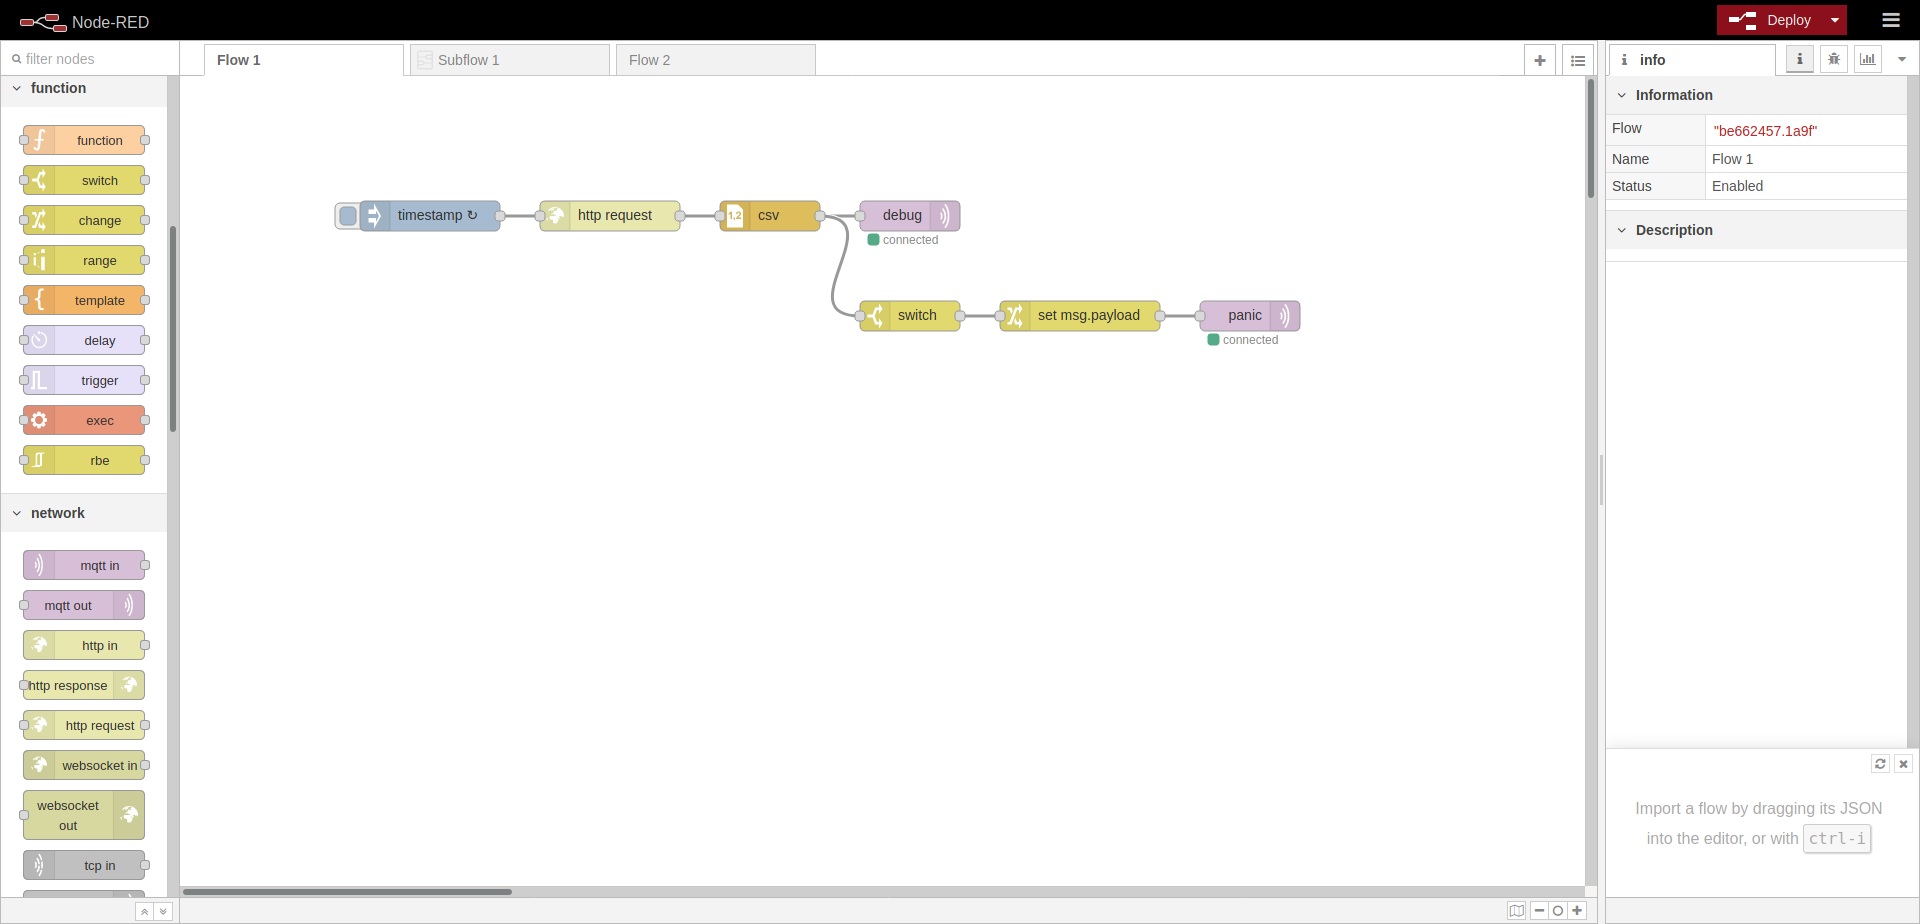
\includegraphics[width=1\textwidth]{node_red_window.png}
\caption{Node-RED environment}
\label{fig:node_red_window}
\end{figure}

One example of a \emph{flow} can be seen in picture \ref{fig:node_red_example}, where a request is being made in intervals of 5 minutes to an HTTP URL that returns a CSV with the feed of significant earthquakes in the last 7 day2s. The data from the CSV is then printed to the debug console and, if the magnitude is equal or bigger than 7, the message "PANIC!" is printed to the console. 

\begin{figure}[!ht]
\centering
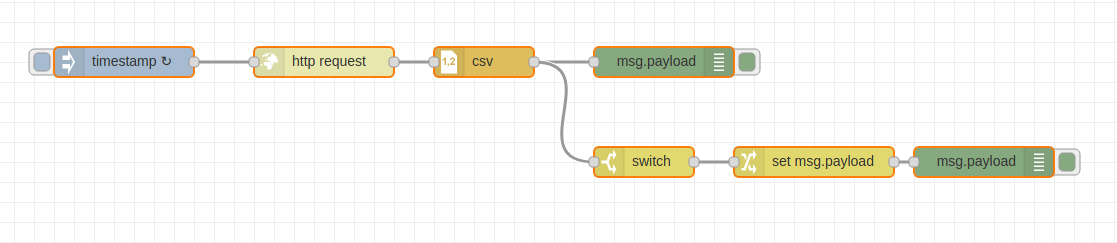
\includegraphics[width=1\textwidth]{node_red_example.png}
\caption{Example of a Node-RED flow}
\label{fig:node_red_example}
\end{figure}

Regarding the architecture of Node-RED, the \texttt{Node} base class is a subclass of Node.js event APIs \texttt{EventEmitter}. This class implements an observer design pattern that maintains a subscriber list of all the nodes connected to it by \emph{wires} and emits events to them. When a node finishes processing data from external sources or another node, it calls the methods \texttt{send()} with a Javascript object. In its turn, this method calls the \texttt{EventEmitter emit()} method that sends named events to the subscribed nodes. 

Being open-source, Node-RED takes advantage of a large community that contributes with new nodes and improvements to the tool. It is the most popular open-source visual programming tool for IoT, with more than 9,300 stars on Github.

\section{Summary}

This chapter introduces two areas that are fundamental to the understanding of this dissertation. Internet-of-Things is defined, as well as its use cases and categories. Fog and Edge computing paradigms are explained, which will be mentioned throughout this document. Node-RED is introduced as a visual programming tool for IoT and its architecture is explained. Finally, a definition and categorization of visual programming languages are introduced and explained.
